\documentclass[crop,tikz]{standalone}
\usetikzlibrary{positioning,arrows,fit,calc}
\pgfdeclarelayer{bg}
\pgfsetlayers{bg,main}
\tikzset{
	>=stealth'
}
\begin{document}
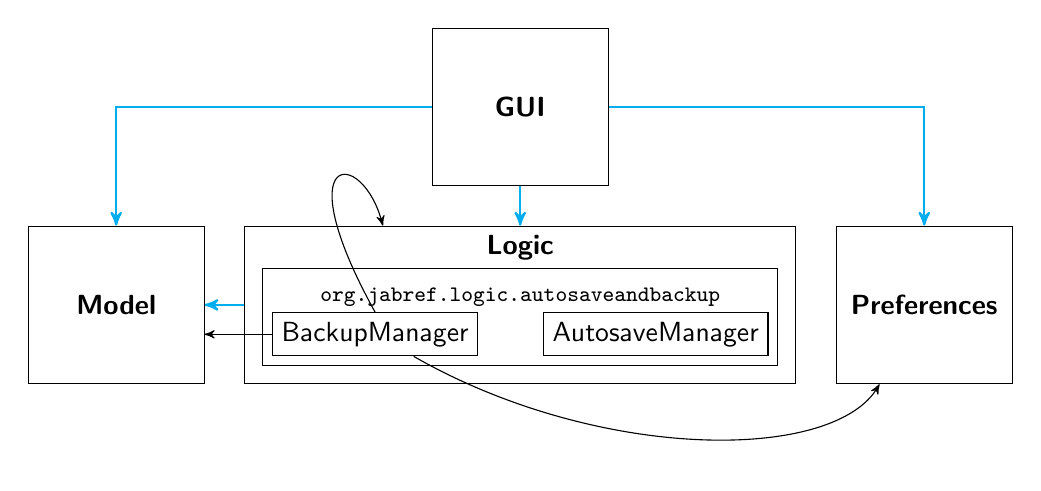
\begin{tikzpicture}[
node distance = 5mm,
every node/.style = {
	font = \sffamily
}, 
component title/.style = {
	font = \bfseries\sffamily
},
component/.style = {
	component title,
	draw, 
	minimum height = 2cm,
	text width = 2cm,
	align = center
},
cmpdep/.style = {
	->,
	thick,
	cyan
},
pkg/.style = {
	font = \footnotesize\ttfamily
}
]

\node [component, minimum width=7cm] (logic) {};
\node [component title, below = 0mm of logic.north] {Logic};

\node [above right = of logic.south west, draw] (bm) {BackupManager};
\node [above left = of logic.south east, draw] (am) {AutosaveManager};

\node [pkg, yshift=1mm] (pkg) at (logic) {org.jabref.logic.autosaveandbackup};
\node [fit=(pkg)(bm)(am), draw] {};

\node [component, left = of logic] (model) {Model};
\node [component, right = of logic] (pref) {Preferences};

\node [component, above = of logic] (gui) {GUI};

\draw[->] (bm.north) .. controls (-3,2) and (-2,2) .. (logic.150);
\draw[->] (bm) -- (bm -| model.east);
\draw[->] (bm) .. controls (1, -2) and (4,-2) .. (pref);

\draw[cmpdep] (logic) -- (model);
\draw[cmpdep] (gui) -| (model);
\draw[cmpdep] (gui) -- (logic);
\draw[cmpdep] (gui) -| (pref);

\end{tikzpicture}

\end{document}